\section{Auswertung}
\label{sec:Auswertung}

Die Messungen werden für zwei Heizraten ausgeführt. Im ersten Schritt werden diese beiden Heizraten aus der Temperatur-Zeit-Abhängigkeit bestimmt. Mit einer Ausgleichsgeraden durch die gemessenen Daten, können die Heizraten bestimmt werden. Die dazugehörigen Plots sind in Abb. \ref{abb:heiz1} zu sehen. 

Die Werte der beiden Heizraten liegen bei 
\begin{align*}
    b_1 &= \SI{3}{\kelvin\per\minute} \\
    b_2 &= \SI{1}{\kelvin\per\minute}. \\
\end{align*}
Die Temperaturen zur Zeit $t=0$ sind an dieser Stelle irrelevant, werden der Vollständigkeit halber aber trotzdem angegeben mit 
\begin{align*}
    T_\text{Start, 1} &= \SI{3}{\kelvin\per\minute} \\
    T_\text{Start, 2} &= \SI{1}{\kelvin\per\minute}. \\
\end{align*}

\begin{figure}
    \centering
    \includegraphics[width=0.8\textwidth]{example-image}
    \caption{Die Temperatur-Zeit-Abhängigkeit bei der Messung. Es wird alle dreißig Sekunden eine Temperatur aufgenommen. Die erste Heizrate ergibt sich zu \SI{3}{\kelvin\per\minute}, die andere liegt bei \SI{1}{\kelvin\per\minute}.}
    \label{abb:detector}
\end{figure}

In Abb. \ref{abb:strom1} und Abb. \ref{abb:strom2} sind die Strom-Temperaturkurven angegeben. Der gemessene Strom hat dabei die Größenordnung \num{e-12} Ampere. Zur Bereinigung des Untergrunds wird eine Exponentialfunktion der Form 
\begin{equation*}
f(x) = a * \exp\left(x b\right)
\end{equation*}  
an die Werte im Bereich außerhalb des Peaks gefittet und von den gesamten Daten abgezogen. Die Fitparameter, die sich dadurch ergeben sind 
\begin{align*}
    a_{1} &= \SI{0}{\pico\ampere} \\
    b_{1} &= \SI{0}{\kelvin} \\
    a_{2} &= \SI{0}{\pico\ampere} \\
    b_{2} &= \SI{0}{\kelvin}. \\
\end{align*}

\begin{figure}
    \centering
    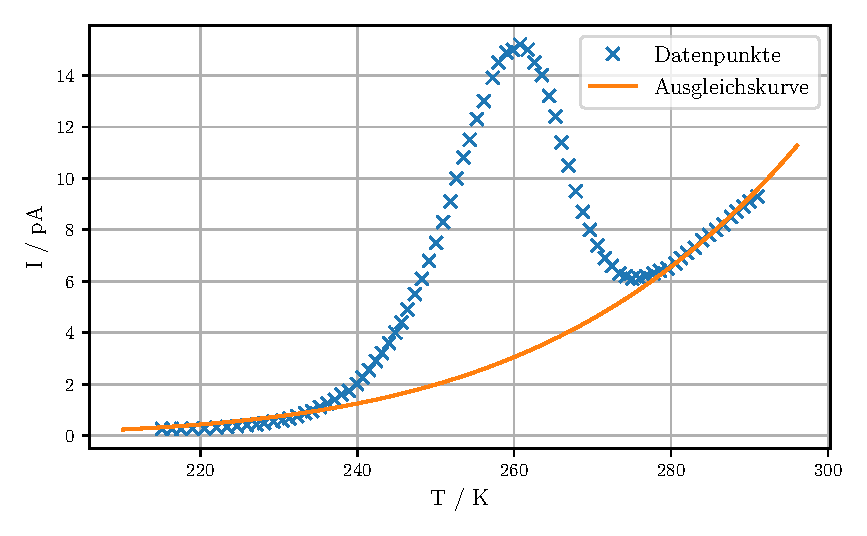
\includegraphics[width=0.8\textwidth]{figures/data_w_bkg1.pdf}
    \caption{}
    \label{abb:strom1}
\end{figure}

\begin{figure}
    \centering
    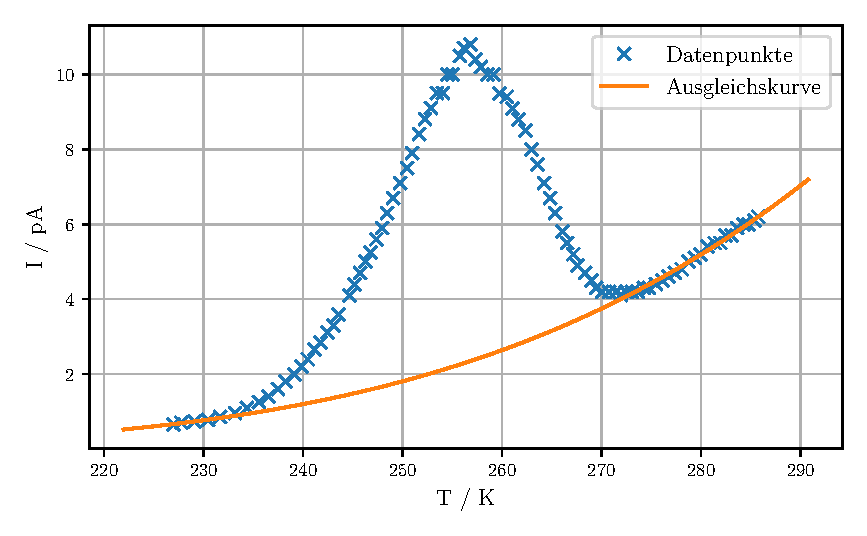
\includegraphics[width=0.8\textwidth]{figures/data_w_bkg2.pdf}
    \caption{}
    \label{abb:strom2}
\end{figure}

Nach der Subtraktion des Untergrunds entstehen die beiden in Abb. \ref{abb:wo_bkg1} und Abb. \ref{abb:wo_bkg2} in denen durch die Variation der Farben erklärt ist, welche Werte für welches Verfahren im folgenden genutzt werden. Die orangenen Werte werden für die Ermittlung der Energie durch die Näherung im Bereich der Anlaufkurve mit Gleichung \eqref{eq:anlauf} genutzt und der gesamte Bereich aus orangenen und grünen Datenpunkten wird für das Integral-Verfahren mit Gleichung \eqref{eq:integral} verwendet. 

\begin{figure}
    \centering
    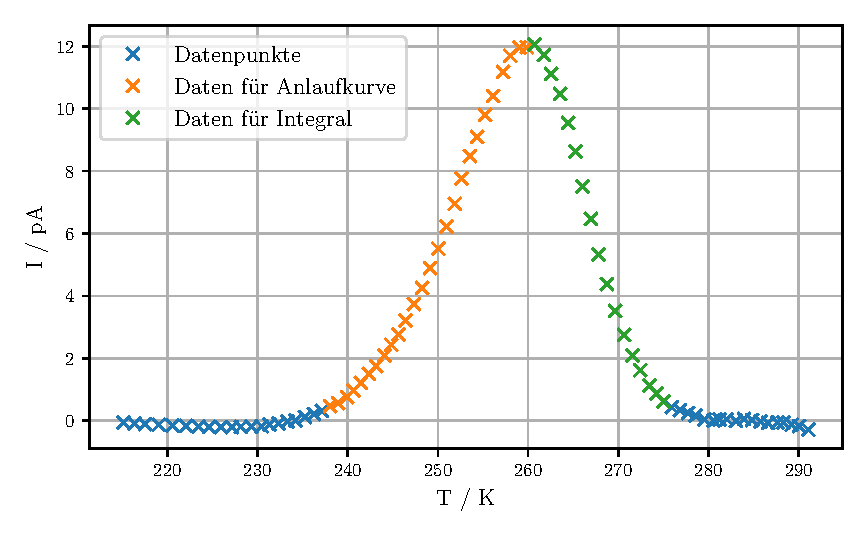
\includegraphics[width=0.8\textwidth]{figures/data_wo_bkg1.pdf}
    \caption{}
    \label{abb:wo_bkg1}
\end{figure}

\begin{figure}
    \centering
    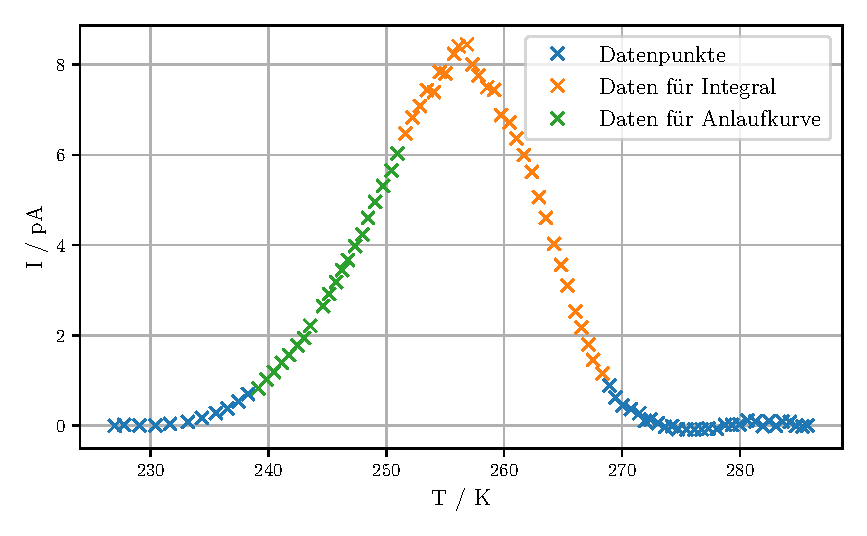
\includegraphics[width=0.8\textwidth]{figures/data_wo_bkg2.pdf}
    \caption{}
    \label{abb:wo_bkg2}
\end{figure}

Die orangenen Werte werden also als Gerade gegen die inverse Temperatur gefittet. Der sich daraus ergebende Wert ist bereits proportional zur Energie, muss aber noch mit der Boltzmann Konstante multipliziert werden, damit er der Energie entspricht. Die Steigung $m$ der Geraden und deren y-Achsenabschnitt $n$ ergeben sich zu 
\begin{align*}
    m_{1} &= \SI{0}{\kelvin} \\
    n_{1} &= \SI{0}{\kelvin} \\
    m_{2} &= \SI{0}{\kelvin} \\
    n_{2} &= \SI{0}{\kelvin}. \\
\end{align*}
Somit liegen die beiden Energien, die sich daraus ergeben bei 
\begin{align*}
    W_{1} &= \SI{0}{\kelvin} \\
    W_{2} &= \SI{0}{\kelvin}. \\
\end{align*}
Die Werte und die Ausgleichsgeraden sind in Abb. \ref{abb:anlauf1} und Abb. \ref{abb:anlauf2} dargestellt. 

\begin{figure}
    \centering
    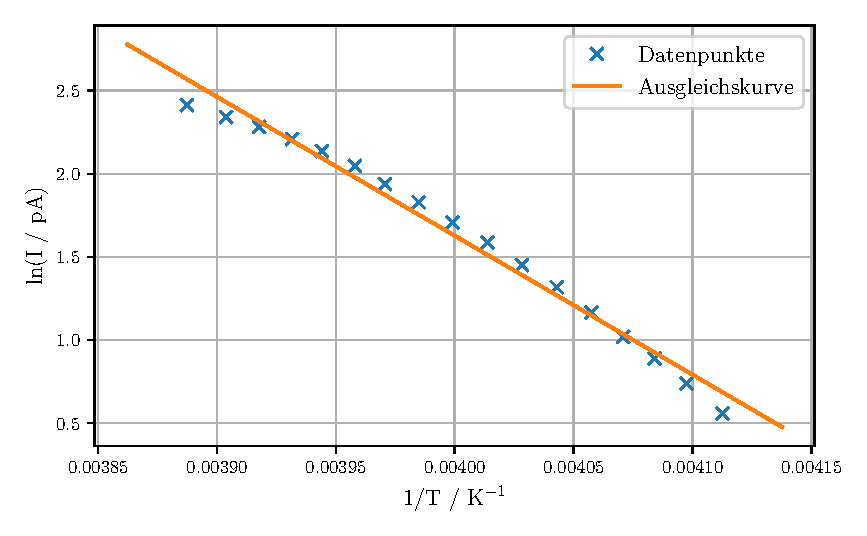
\includegraphics[width=0.8\textwidth]{figures/anlauf1.pdf}
    \caption{}
    \label{abb:anlauf1}
\end{figure}

\begin{figure}
    \centering
    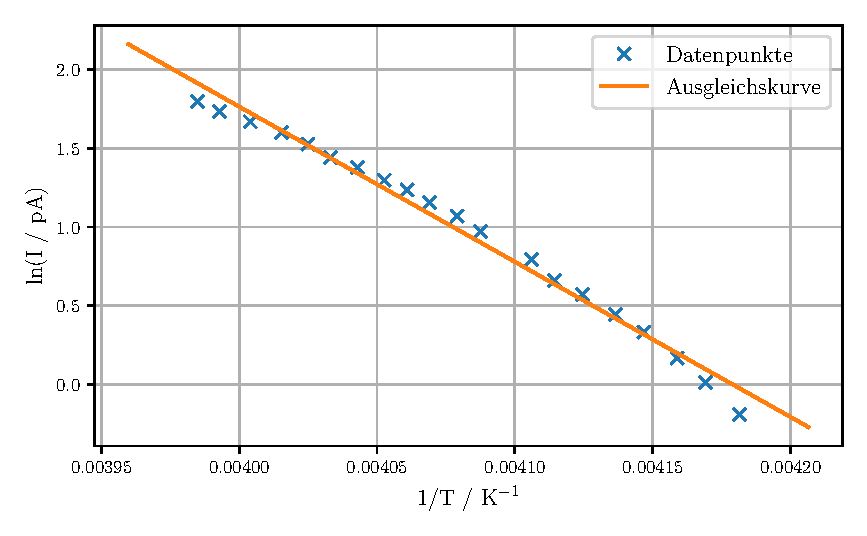
\includegraphics[width=0.8\textwidth]{figures/anlauf2.pdf}
    \caption{}
    \label{abb:anlauf2}
\end{figure}

Das Integralverfahren nach Gleichung \eqref{eq:integral} wird mithilfe der Simpson Regel ausgeführt. Der Bereich der orangenen und grünen Werte wird dabei Schrittweise integriert und entsprechend der Gleichung ergibt sich dann ein linearer Zusammenhang.
Aus der ermittelten Steigung lässt sich erneut die Energie bestimmen. Die Werte und Geraden sind in Abb. \ref{abb:integral1} und \ref{abb:integral2} dargestellt. Die Werte die sich durch die Ausgleichsrechnung ergeben sind 
\begin{align*}
    m_{1} &= \SI{0}{\kelvin} \\
    n_{1} &= \SI{0}{\kelvin} \\
    m_{2} &= \SI{0}{\kelvin} \\
    n_{2} &= \SI{0}{\kelvin} \\
\end{align*}
und die beiden Energien, die sich daraus ergeben sind 
\begin{align*}
    W_{1} &= \SI{0}{\kelvin} \\
    W_{2} &= \SI{0}{\kelvin}. \\
\end{align*}

Mithilfe der ermittelten Energien ergibt sich über Gleichung \eqref{eq:tmax} und die Temperaturen bei den Maxima der Kurven, die bei 
\begin{align*}
    W_{1} &= \SI{0}{\kelvin} \\
    W_{2} &= \SI{0}{\kelvin} \\
\end{align*}
liegen, die Zeit $\tau_0$ für beide Heizraten. Da vier relativ verschiedene Werte für die Energien $W$ bestimmt wurden, ergeben sich daraus auch vier verschiedene Werte für $\tau_0$.
Die Werte sind 
\begin{align*}
    m_{1} &= \SI{0}{\kelvin} \\
    n_{1} &= \SI{0}{\kelvin} \\
    m_{2} &= \SI{0}{\kelvin} \\
    n_{2} &= \SI{0}{\kelvin}. \\
\end{align*}

Die aus den Zeiten $\tau_0$ resultierenden Kurven nach Gleichung \eqref{eq:tau} sind in Abb. \ref{abb:tau} dargestellt.



